\documentclass[11pt,letterpaper]{article}
\usepackage{emnlp2017}
\usepackage{times}
\usepackage{url}
\usepackage{latexsym}
\usepackage{graphicx}
\usepackage{setspace}

\emnlpfinalcopy % System descriptions should not be anonymous

\title{Classifier Stacking for Native Language Identification}

\author{Wen Li \\
  Department of Linguistics \\
  Indiana University \\
  Bloomington, IN, USA \\
  {\tt wl9@indiana.edu} \\\And
  Liang Zou \\
  Department of Mathematics \\
  Indiana University \\
  Bloomington, IN, USA \\
  {\tt liazou@indiana.edu} \\}

\date{}

\begin{document}
\maketitle
\begin{abstract}
%This document contains the instructions for preparing a camera-ready system description paper for the NLI 2017 shared task.
This paper reports our contribution (team WLZ) to the NLI Shared Task 2017 (essay track). We first extract lexical and syntactic features from the essays, perform feature weighting and selection, and train linear support vector machine (SVM) classifiers each on an individual feature type. The output of base classifiers, as probabilities for each class, are then fed into a multilayer perceptron to predict the native language of the author. We also report the performance of each feature type, as well as the best features of a type. Our system achieves an accuracy of 86.55\%, which is among the best performing systems of this shared task.
%\bf Please write a brief \emph{abstract} describing your system and the results you obtained (list the best results in each track). You can also briefly mention any insights or interesting highlights from your results.

\end{abstract}

\section{Introduction}
\label{intro}

Native language identification (NLI) is the task of determining an author's native language (L1) based on their writings in a second language (L2). NLI works under the assumption that an author's L1 will dispose them towards particular language production patterns in their L2, as influenced by their native language. This relates to cross-linguistic influence (CLI), a key topic in the field of second language acquisition (SLA) that analyzes transfer effects from the L1 on later learned languages \cite{malmasi2016}. The identification of L1-specific features has been used to study language transfer effects in second-language acquisition \cite{malmasi2014}, which is useful for developing pedagogical material, teaching methods, L1-specific instructions and generating learner feedback that is tailored to their native language.

The first NLI shared task was held in 2013 \cite{nli2013}, and the winner team reported an accuracy of 83.6\% on the test data using an SVM classifier with over 400,000 unique features consisting of lexical and POS $n$-grams occurring in at least two texts in the training set \cite{jarvis-bestgen-pepper:2013:BEA8}. In addition to $n$-gram features, other researchers have also explored syntactic features \cite{bykh:2014} and the use of string kernels \cite{ionescu:2014}.

All NLI shared tasks to date have been based on L2 English data, but NLI research has been extended to at least six other non-English languages \cite{multilingual-nli}. In addition to using the written responses, a recent trend has been the use of speech transcripts and audio features for dialect identification \cite{vardial2016}. The combination of transcripts and acoustic features has also provided good results for dialect identification \cite{vardial2017}. Following this trend, the 2016 Computational Paralinguistics Challenge \cite{compare2016} also included an NLI task based on the spoken response. The NLI Shared Task 2017 attempts to combine these approaches by including a written response (essay) and a spoken response (speech transcript and i-vector acoustic features) for each subject. The task also allows for the fusion of all features.

Ensemble methods using multiple classifiers have proven to be one of the most successful approaches for the task of NLI \cite{malmasi:2017:nlisg}, and researchers have reported better results using stacking than a single classifier in other text classification tasks \citep[e.g.,][]{liu2016}. In this work we present a stacking model using lexical and syntactic features for NLI Shared Task 2017 \cite{nli2017}, report the performance of different feature types, and show the best features in each type. The features we use in the final model include character/word/stem $n$-grams, function word $n$-grams, and dependency parses.

\section{Data}
The data set we use for NLI Shared Task 2017 \citep[see details in][]{nli2017} includes English essays written by test takers who participated in a standardized assessment of English proficiency for academic purposes. The 11 native languages of the test takers are: Arabic (ARA), Chinese (CHI), French (FRE), German (GER), Hindi (HIN), Italian (ITA), Japanese (JPN), Korean (KOR), Spanish (SPA), Telugu (TEL), and Turkish (TUR). There are 11,000 essays (1,000 per L1) in the training partition (Train), 1,100 (100 per L1) in the development partition (Dev), and 1,100 (100 per L1) in the test partition (Test). All essays are available in both original and tokenized texts.

\section{Methods}
\subsection{Features}
We use \textbf{tf-idf weighting} for all the features in this work, since we observe better results than other feature representations, namely binary representation and frequency-based representation. For most of the feature types, we also \textbf{select $k$-best features} with chi-square metric instead of using all of them. Previous research has reported feature selection could improve the classification accuracy \cite{liu2014}, and we notice the same trend for this task. In preliminary experiments feature selection increases the accuracy by around 1\-3\% for each feature type. The $k$ value for each feature type varies with regard to the total number of features, and we choose the selected number of features based on their performance on the Dev set (trained on Train set). Both tf-idf weighting and feature selection are realized with Scikit-Learn \cite{sklearn}.

\paragraph{Character $n$-grams}
We extract character 3-7 grams from the tokenized text, and each is represented as a feature type (denoted by Char3-7). We also experiment with character 8-9 grams but do not include them in the final model, since adding them does not improve the accuracy.

\paragraph{Word $n$-grams}
We extract word uni-, bi-, and tri-grams from the tokenized text, and each is represented as a feature type (denoted by Word1-3).

\paragraph{Lemma $n$-grams}
We use the WordNet Lemmatizer in NLTK \cite{nltk} to lemmatize the tokenized essays, and then extract lemma uni-, bi-, and tri-grams as feature types (denoted by Lemma1-3). However, we do not include these features in the final model, since adding them does not improve the accuracy.

\paragraph{Stem $n$-grams}
We first stem the tokenized text with Porter stemmer using NLTK, and then extract stem uni-, bi-, and tri-grams as feature types (denoted by Stem1-3).

\paragraph{POS $n$-grams}
We use the Stanford POS tagger \cite{tagging} to tag the tokenized essays, and then extract POS uni-, bi-, and tri-grams as feature types (denoted by POS1-3). However, we do not include these features in the final model, since adding them does not improve the accuracy.

\paragraph{Function word $n$-grams}
We use the Stanford POS tagger to tag the tokenized essays first, and then extract the function words by their POS tags (which are tagged as auxiliary verbs, conjunctions, determiners, pronouns, etc.). Function word uni-, bi-, and tri-grams are used as features (denoted by FW1-3).

\paragraph{Dependency parses}
We use the Stanford dependency parser \cite{parsing} to extract the dependencies from the tokenized essays. Three types of dependencies are included in the experiments (taking ``I agree" as an example): original dependency (Dep0), e.g., (agree, nsubj, I); dependency where one of the word is replaced by its POS tag (Dep1), e.g., (VBP, nsubj, I) and (agree, nsubj, PRP); dependency where both of the words are replaced by their POS tags (Dep2), e.g., (VBP, nsubj, PRP). We include the POS-replaced dependencies, since we believe they would generalize better, as noted by \citet{malmasi:2017:nlisg}.

\paragraph{Word embeddings}
We use the Common Crawl (42B tokens, 1.9M vocab, uncased, 300d vectors) in GloVe (global vectors for word representation) \cite{glove} to produce feature vectors for each essay, with the help of Gensim \cite{gensim}. For all the words in an essay, we average their word vectors if they occur in the GloVe vocabulary as well. We observe that word vectors with larger dimension perform better than those with lower dimension when experimenting with different dimensions (e.g., 50d, 100d, 200d, 300d). However, we do not include the word embedding features (denoted by WV300) in the final model, since adding them does not improve the accuracy.

\begin{table*}[h]
\center
\begin{tabular}{|c|rr|ccc|}
\hline
\bf Feature type & \bf Total \# & \bf Selected \# & \bf CV & \bf Dev & \bf Test \\
\hline
Char3 & 11,320 & 10,000 & 0.7327 & 0.7447 & 0.7555 \\
Char4 & 51,072 & 30,000 & 0.7944 & 0.7827 & 0.8145\\
Char5 & 145,575 & 30,000 & 0.8158 & 0.8045 & 0.8264 \\
Char6 & 334,117 & 30,000 & 0.8260 & 0.8000 & 0.8309 \\
Char7 & 631,139 & 50,000 & 0.8386 & 0.8018 & \bf 0.8336 \\
\hline
Word1 & 25,950 & 20,000 & 0.7699 & 0.7627 & 0.8136 \\
Word2 & 205,625 & 50,000 & 0.8417 & 0.7809 & \bf 0.8245 \\
Word3 & 384,184 & 50,000 & 0.8227 & 0.7082 & 0.7218 \\
\hline
Stem1 & 145,575 & 10,000 & 0.7572 & 0.7618 & 0.7827 \\
Stem2 & 334,117 & 30,000 & 0.8276 & 0.7791 & \bf 0.8118 \\
Stem3 & 631,139 & 30,000 & 0.7982 & 0.6964 & 0.7127 \\
\hline
FW1 & 511 & all & 0.4199 & 0.4309 & 0.4227 \\
FW2 & 12,385 & all & 0.4623 & 0.4764 & \bf 0.4900 \\
FW3 & 104,770 & all & 0.4174 & 0.4300 & 0.4464 \\
\hline
Dep0 & 253,719 & 30,000 & 0.7868 & 0.6718 & 0.7473 \\
Dep1 & 256,271 & 30,000 & 0.7996 & 0.7336 & \bf 0.7709 \\
Dep2 & 4,426 & 4,000 & 0.4598 & 0.4645 & 0.4745 \\
\hline
\hline
Lemma1 & 22,541 & 20,000 & 0.7614 & 0.7627 & -- \\
Lemma2 & 181,533 & 50,000 & 0.8389 & 0.7891 & -- \\
Lemma3 & 355,414 & 50,000 & 0.8242 & 0.7082 & -- \\
\hline
POS1 & 44 & all & 0.3516 & 0.3800 & -- \\
POS2 & 12,385 & all & 0.5297 & 0.5173 & -- \\
POS3 & 18,961 & 15,000 & 0.5741 & 0.5710 & -- \\
\hline
WV300 & 300 & 300 & 0.5645 & 0.5673 & -- \\
\hline
\end{tabular}
%TODO : you should write a descriptive caption
\caption{Total number of features, selected number of features, and accuracy of each feature type. CV: 10-fold cross validation on Train; Dev: trained on Train, tested on Dev; Test: trained on Train and Dev, tested on Test. Best performance of a feature group on Test is in bold.}
\label{tab:results-1}
\end{table*}


\subsection{Classifiers}
We use \textbf{linear SVM} (implemented by Scikit-Learn) as the base classifier for the feature types mentioned above. We set C=0.8 for Char3, Word1, Stem1, FW1-3, and Dep2, and use default settings for other parameters. Experiments on other feature types use the default setting: C=1.0, L2 penalty, squared hinge loss, etc. For each feature type, we run 10-fold cross validation on Train and test on Dev to decide the number of selected features we would like to use for the final system. 

To combine the output of probabilities from base classifiers and predict the final label, one method is to concatenate all the probabilities and feed into a classifier to generate the final prediction. We examine the performance of \textbf{multilayer perceptron} (MLP), linear SVM, Linear Discriminant Analysis (LDA), and MLP performs the best. We try different hidden layer sizes, and finally use one hidden layer of 100 perceptrons. Since MLP produces different results in every run, our final results using MLP contains the average results of 10 runs to reduce the variance.

We also try combining the probabilities mathematically: 1) summing up the probabilities from all feature types and taking the maximum as final prediction (denoted by SumProbs); 2) summing up the logarithmized probabilities from all feature types and taking the maximum as final prediction (denoted by LogSumProbs).

We run cross validation on Train and Dev to decide which feature types to include in the final model.


\section{Results}
\label{sec:results}

\subsection{Results by feature type}
We report the performance of each feature type in Table \ref{tab:results-1}. The upper part contains the 17 features we use in the final model, and the lower part contains some features we would like to explore but do not include in the final submissions. 

We can see that the total number of features is very large for some feature types, which makes feature selection necessary. However, we choose the number of features by their performance on Dev and cross validation on Train, so there is no guarantee that we have the optimal number of selected features.

The features that perform comparatively well on Test set are: Char7, Word2, Stem2, FW2, and Dep1. We believe that bigrams perform better than unigrams or trigrams in general, because they consider context more than unigrams and generalize better than trigrams.

We also show the top features for each feature type ranked by Chi-square in Table \ref{tab:results-4}, in the hope that it would be helpful for  researchers interested in SLA or at least provide some insights to the readers. We notice that among the word $n$-grams are some country related words such as ``italy'' and ``in japan'', as well as some common expressions such as ``in order to'' and ``more and more''.

\subsection{Final results}
The Word Unigram baseline in Table \ref{tab:results-2} is achieved by using normalized frequency of all the word unigrams (which occurred at least three times in the essays) as features, and linear SVM as the classifier. 

We try different methods of combining the output of probabilities by base classifiers and report their performance in Table \ref{tab:results-2}. MLP and linear SVM are the best combiners among our experiments (other classifiers include random forest, LDA, logistic regression). When not using a classifier, summing up the logarithmized probabilities achieves better results than summing up the probabilities directly. The detailed evaluation of our best performing system is shown in Table \ref{tab:results-3}, and the confusion matrix is shown in Figure \ref{fig:1}.

From the confusion matrix we observe a few quite distinctive language groups: CHI, JPN, and KOR; HIN and TEL; FRE, ITA, and SPA. We suppose the confusion between languages results more from cultural than linguistic reasons. For instance, HIN and TEL are mutually misclassified in a lot of cases, while HIN belongs to Indo-European language family and TEL belongs to Dravidian. Similarly, CHI, JPN, and KOR come from three different language families, but they are in a cluster where one is often misclassified as another. 

\begin{table}[h!]
\center
\begin{tabular}{|l|cc|}
\hline
\bf System & \bf F1 (macro) & \bf Accuracy \\
\hline
Random Baseline & 0.0909 & 0.0909 \\
Word Unigram & 0.7104 & 0.7109 \\
\hline
MLP & \bf 0.8654 & \bf 0.8655 \\
LinearSVM & 0.8593 & 0.8591 \\
LogSumProbs & 0.8564 & 0.8565 \\
SumProbs & 0.8554 & 0.8555 \\
LDA & 0.8446 & 0.8445 \\
\hline
\end{tabular}
%TODO : you should write a descriptive caption
\caption{Final results using different combining methods. Trained on Train and Dev, tested on Test.}
\label{tab:results-2}
\end{table}

\begin{table}[h!]
\center
\begin{tabular}{|c|ccc|}
\hline
& \bf Precision & \bf Recall & \bf F1 \\
\hline
        ARA  &   0.8673  &  0.8500  &  0.8586       \\
        CHI  &   0.9388  & 0.9200  &  0.9293       \\
        FRE   &  0.8600  &  0.8600  &  0.8600       \\
        GER   &  0.9406  &  0.9500   & \bf 0.9453       \\
        HIN   &  0.7843  &  0.8000  &  \textit{0.7921}       \\
        ITA   &  0.8878  &  0.8700  &  0.8788       \\
        JPN   &  0.8679  &  0.9200  &  0.8932       \\
        KOR  &   0.8632  &  0.8200  &  0.8410       \\
        SPA   &  0.8173  &  0.8500  &  0.8333       \\
        TEL   &  0.8265   & 0.8100  &  0.8182     \\
        TUR   &  0.8700  &  0.8700  &  0.8700   \\
\hline
avg / total   &  0.8658  &  0.8655  &  0.8654 \\
\hline
\end{tabular}
%TODO : you should write a descriptive caption
\caption{Detailed evaluation of our best performing system. Trained on Train and Dev, tested on Test. Best and worst F1 in bold and italics.}
\label{tab:results-3}
\end{table}

\begin{figure*}
\centering
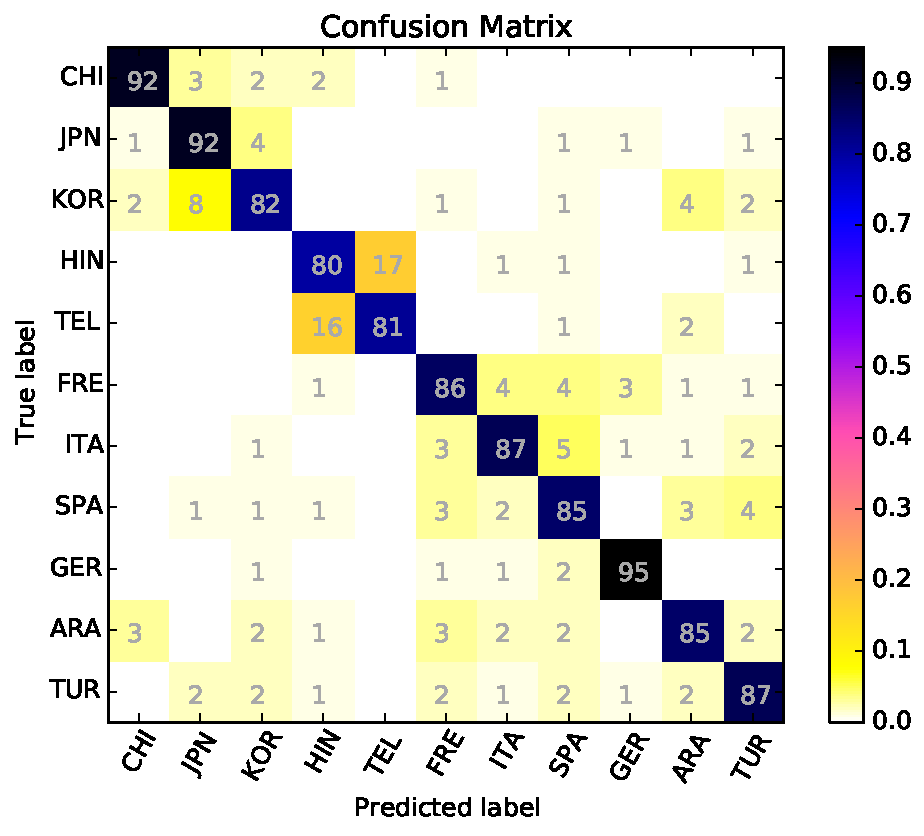
\includegraphics[width=0.7\textwidth]{confusion_matrix.pdf}
%TODO : add your own details to the caption for this figure
\caption{Confusion matrix of our best performing model.}
\label{fig:1}
\end{figure*}

\section{Discussion and future work}

We explore the performance of different feature types for NLI in this work. Among the features types we examine, character/word/lemma/stem $n$-grams have the best individual performance. Dependency parses are also informative with respect to the native language of the author. POS $n$-grams might be too general for this task, achieving around 50\% accuracy alone. Word embeddings are good indicators for text classification tasks such as sentiment analysis, which relies heavily on the semantics of the content. NLI is not only about the semantics of the text but also involves writing style (e.g., the use of expressions and sentence structure). We suppose this justifies the performance of using word embeddings as features.

When we combine the output of base classifiers using different feature types to predict the final label, we have to decide which feature types to include. It is not practical to try all the combinations of features, so we start with the feature types with best individual performance, adding one and another. We do not include a feature type if it does not improve the accuracy on cross validation, and thus we cannot guarantee the optimization of performance on the test data. This process is very time consuming, and we believe there should be a better way of doing so. At the same time we observe adding lemma $n$-grams does not help, although lemma $n$-grams achieve very high accuracy by themselves. We believe the reason is that lemma $n$-grams are overlapping with word $n$-grams a lot, so they do not contribute more to the final prediction. We should keep in mind that good classifiers for ensemble learning need both accuracy and diversity. It remains unclear why function words (with accuracy of around 40\%-50\%) help more than POS $n$-grams or word embeddings, though.

We notice MLP improves the system performance over linear SVM as a combiner. For an individual feature type, MLP also performs better than linear SVM in most cases; however, we choose linear SVM as the base classifier, since it has better balance between speed and accuracy. MLP is roughly ten times slower than linear SVM when we run the experiments. This points us to the use of neural networks, since MLP is one of the simplest neural architecture. We would like to explore more about neural networks for NLI in future. 

Another direction of future work may be towards a different architecture of combing various feature types. Ensemble methods have been studied quite a lot in text classification tasks; however, building an ensemble classifier is hardly an end-to-end task. We would like to explore how we can make the system smarter and learn by itself with less human input.

Finally, we hope the work in NLI would be of interest to the researchers from SLA/ESL. We hope the work we have done for NLI could be potentially useful for language teachers, and we would like to collaborate with them if they need anything from the view of computational linguistics.

\cleardoublepage
\begin{table*}[t]
\scriptsize
\center
\begin{tabular}{|c|p{138mm}|}
\hline
\bf Feature Type & \bf Top Features Selected by Chi-square \\
\hline
Char3 & h; vel; ink; n j; alo; pan; -t ; oup; oft; u w; owe; . .; kyo; fue;  u ; nk ;  'm; 'm ;  a ; he ; i '; u a;  - ;  \& ;  ..; , i;  .
; gst; yme; i t;  i ; wev; ho;  gu; oym;  yo; apa; you; gui; uid; tou;  : ; rav;  , ;  ja; urk;  ko; ou ; kor; jap \\
\hline
Char4 & veli; ticu; germ; gste; ngst; ften; ofte; bbli; owev; weve; lopp; nk t; ymen; . ho; how; , i ; i th; oyme; ur g;  you; r gu; pane;  gui; joym; rkey; urke; guid; uide;  tou; rave; deed; avel; trav;  ita; ndee; in j; tour; ind; n ko; turk; pan ; alot; n ja; you ; orea;  kor; kore;  jap; apan; japa \\
\hline
Char5 & i thi; n ita; avel ; rean ; eed ,; oymen; 
howe; our g; k tha; orean; r gui; ur gu; rkey ; joyme; turke; urkey; uide ; njoym;  guid; guide;  in j; panes; pan ,; apane; ravel; anese; trave; deed ;  trav;  ital; indee; ndeed;  tour; tour ; .
ind;  turk; in ko; n kor; inde;  alot; alot ; orea ; in ja;  you ; n jap; apan ;  kore; korea;  japa; japan \\
\hline
Char6 & a tour; ravel ; eed , ; orean ; . howe; oyment; howev; orea ,; k that; nk tha; korean; r guid; ur gui; our gu; urkey ;  turke; joymen; turkey; njoyme; enjoym; guide ;  guide; tour g; pan , ; apanes; japane; anese ; apan ,; panese; travel;  trave; indeed; ndeed ;  in ko;  . ind; deed ,;  tour ; in kor; n kore; . inde; indee;  in ja; alot o;  alot ; korea ; n japa; japan ; in jap;  korea;  japan \\
\hline
Char7 & wever ,;  a tour; a tour ; travel ; oyment ; . howev;  . howe; korean ; howeve; k that ; korea ,; orea , ; nk that; ink tha;  korean;  enjoym; r guide; ur guid; our gui; turkey ;  turkey; tour gu; joyment; njoymen; enjoyme;  guide ;  tour g;  japane; japanes; apan , ; japan ,; panese ; indeed ;  travel; apanese; deed , ;  in kor; ndeed ,; in kore;  . inde; . indee; n korea; indeed;  alot o;  in jap; alot of;  korea ; n japan; in japa;  japan \\
\hline
Word1 & u; jack; developped; infact; milan; pubblic; exemple; preparation; trip; 'm; youth; group; \&; think; the; your; various; france; dont; ..; -; a; youngsters; he; germany; hence; his; italy; towards; traveling; particular; italian; often; however; thier; travel; i; korean; guide; enjoyment; turkey; :; japanese; indeed; tour; ,; alot; korea; you; japan \\
\hline
Word2 & {and hence; that you; jack of; the youth; it 's; led by; younger generation; the above; , they; when compared; i 'm; a particular; group tour; you are; first ,; two reasons; a group; particular subject; korea .; in germany; second ,; now a; , we; . second; japan .; as compared; , and; . ..; , that; in fact; i conclude; in italy; where as; in france; in turkey; a days; . however; i think; a tour; , i; however ,; think that; korea ,; tour guide; japan ,; indeed ,; in korea; . indeed; alot of; in japan } \\
\hline
Word3 &  a lot of; have alot of; of all ,; conclude , i; , young people; master of none; , i think; tour guide .; enjoy a lot; , they can; , in japan; usage of cars; of all trades; . i think; the younger generation; to conclude ,; on the one; each and every; the possibility to; i feel that; a group led; . therefore ,; however , i; reasons , i; the one hand; group led by; . to conclude; . in japan; for this reason; is , that; i conclude that; in korea .; jack of all; led by a; when compared to; . first ,; in a group; by a tour; are two reasons; . in fact; . second ,; in japan .; as compared to; a tour guide; now a days; in korea ,; . however ,; in japan ,; i think that; . indeed ,\\
\hline
Stem1 & atleast; an; that; istanbul; intrest; taiwan; india; commun; fuel; tokyo; trip; group; infact; possibl; jack; milan; think; toward; advertiss; difer; the; exempl; youth; dont; variou; your; he; franc; hi; henc; germani; itali; particular; pubblic; youngster; often; thier; howev; italian; korean; guid; turkey; travel; japanes; tour; inde; alot; korea; you; japan \\
\hline
Stem2 & all trade; when you; with out; have alot; feel that; you will; the italian; usag of; old age; each and; one hand; in india; peopl that; master of; group led; you have; mode of; to conclud; conclud that; and henc; everi thing; that you; when compar; possibl to; the youth; in group; jack of; younger gener; the abov; led by; enjoy lot; the subject; particular subject; you are; group tour; in germani; by tour; two reason; as compar; in fact; now day; in itali; where as; in franc; in turkey; think that; tour guid; in korea; alot of; in japan \\
\hline
Stem3 & the new thing; alot of money; alot of thing; the statement that; and for thi; in olden day; youth of today; are my follow; in order to; the youth of; in today world; would say that; for these reason; for exampl consid; the older peopl; day by day; in thi way; for new thing; mode of transport; when you are; think that is; final conclud that; the usag of; accord to me; to my mind; all the subject; travel in group; the young peopl; more and more; you have to; think that in; tri for new; have alot of; master of none; usag of car; in group led; each and everi; the possibl to; on the one; of all trade; the younger gener; the one hand; group led by; for thi reason; jack of all; when compar to; led by tour; by tour guid; are two reason; as compar to \\
\hline
FW1 & when; whether; to; about; by; some; amongst; it; can; into; every; than; there; atleast; must; three; across; or; why; upon; she; till; because; behind; will; could; of; though; my; would; whereas; might; they; their; this; him; that; olden; any; the; we; its; an; may; which; your; he; his; towards; you \\
\hline
FW2 & that why; the he; all the; there three; you in; and he; some might; one should; to you; the may; the behind; any one; that that; that this; that in; you the; because you; his and; and that; you you; of the; which he; it to; you and; they can; what you; and towards; the which; he can; and you; he will; towards the; by myself; every one; in by; in olden; there two; he may; we can; in his; towards their; if you; you can; the you; you will; the of; when you; where as; that you; you to \\
\hline
FW3 & some might that; there three as; you to and; as as with; the towards their; all but of; the of an; you to in; in the twenty; there in twenty; than there two; the you to; the in olden; some might with; to would that; you will to; you to the; they how to; for us to; you to to; if you to; in to this; but on the; that you can; we can the; the where as; above we can; their towards their; on of that; for these with; the these my; when you you; all as before; and for this; that in the; that you to; where as the; there two for; all in all; in all as; with the that; two for this; we can that; as would that; in the of; to in by; the of the; the that you; on the one; each and every \\
\hline
Dep0 & compared\_advmod\_when; days\_det\_these; student\_det\_the; important\_cop\_; enjoyment\_case\_of; possibility\_det\_the; thing\_det\_every; subjects\_det\_the; taiwan\_case\_in; each\_cc\_and; usage\_nmod\_cars; self\_nmod; enjoy\_dobj\_lot; hand\_nummod\_one; product\_det\_a; subject\_det\_the; knowledge\_det\_a; take\_dobj\_example; group\_acl\_led; conclude\_mark\_to; india\_case\_in; people\_det\_the; generation\_det\_the; feel\_nsubj\_i; generation\_amod\_younger; have\_nsubj\_you; group\_det\_a; preparation\_det\_a; youth\_det\_the; led\_nmod\_guide; reasons\_nummod\_two; tour\_compound\_group; group\_case\_in; subject\_amod\_particular; guide\_case\_by; days\_det\_a; germany\_case\_in; fact\_case\_in; italy\_case\_in; france\_case\_in; turkey\_case\_in; conclude\_nsubj\_i; poss\_his; guide\_det\_a; think\_nsubj\_i; guide\_compound\_tour; korea\_case\_in; japan\_case\_in \\
\hline
Dep1 & nn\_acl\_led; conclude\_mark\_to; nn\_det\_any; led\_nmod\_nn; youth\_det\_dt; generation\_amod\_jjr; vbn\_nmod\_guide; conclude\_nsubj\_fw; vbg\_mark\_in; subject\_det\_dt; group\_det\_dt; enjoyment\_case\_in; vbp\_advmod\_indeed; preparation\_amod\_jj; nn\_case\_towards; group\_case\_in; nn\_det\_a; tour\_compound\_nn; vbp\_nsubj\_that; preparation\_det\_dt; poss\_your; nns\_amod\_various; vbp\_nsubj\_i; nn\_amod\_italian; nns\_det\_the; nn\_nmod\_korea; india\_case\_in; vb\_dobj\_alot; germany\_case\_in; vb\_nsubj\_you; reasons\_nummod\_cd; nn\_amod\_japanese; nn\_nmod\_japan; france\_case\_in; italy\_case\_in; vbd\_nsubj\_i; think\_nsubj\_prp; guide\_case\_in; nn\_amod\_particular; turkey\_case\_in; alot\_nmod\_nn; vbp\_nsubj\_you; guide\_det\_dt; guide\_compound\_nn; alot\_nmod\_nns; nn\_compound\_tour; korea\_case\_in; japan\_case\_in \\
\hline
Dep2 & jjs\_case\_to; vbg\_dobj\_nn; vb\_dobj\_prp; vb\_nsubj\_prp; vbg\_nsubj\_nns; jj\_mwe\_in; vb\_advcl\_vbp; vbp\_ccomp\_jj; vbg\_nmod\_nns; jj\_cop\_vbz; nn\_case\_in; prp\_case\_vbg; jj\_nsubj\_prp; vbd\_dobj\_nn; nn\_compound\_nn; jj\_xcomp\_vb; jjr\_conj\_jjr; vb\_aux\_vbd; vb\_nsubj\_fw; vbp\_nsubj\_wdt; vbd\_advmod\_rb; vbp\_advmod\_rb; jj\_advmod\_rb; predet\_pdt; nn\_nmod\_nn; vbd\_nmod\_nnp; jj\_cop\_vb; nnp\_nmod\_dt; vbp\_expl\_ex; nns\_det; jj\_cop\_vbg; in\_mwe\_nn; vb\_nsubj\_nns; vb\_aux\_vbp; vb\_advmod\_ls; vbn\_aux\_vbz; vb\_neg\_rb; vbd\_nsubj\_fw; poss\_nns; vbg\_mark\_in; jj\_mark\_to; nns\_case\_pos; vbp\_nsubj\_nns; vbp\_nsubj\_prp; vbp\_advmod\_ls; nns\_det\_dt; vbp\_nsubj\_fw; vbd\_nsubj\_prp; nn\_det\_dt \\
\hline
\end{tabular}
\caption{Top features ranked by Chi-square on Train and Dev (separated by ``;'').}
\label{tab:results-4}
\end{table*}


%\section*{Acknowledgements}
% This is an optional section
\cleardoublepage
% \newpage
\bibliography{nli2017}
\bibliographystyle{emnlp_natbib}
\end{document}

%%%%%%%%%%%%%%%%%%%%%%%%%%%%%%%%%%%%%%%%%%%%%%%%%%%%%%%%%%%%%%%%%%
%   Thank you for participating in the NLI 2017 shared task!     %
%                                                                %
%   We look forward to reading your system description papers.   %
%%%%%%%%%%%%%%%%%%%%%%%%%%%%%%%%%%%%%%%%%%%%%%%%%%%%%%%%%%%%%%%%%%
